As a software library grows, so does its complexity. This comment certainly applies to QMCPy \cite{QMCPy2020a}, our Python library for high-dimensional numerical integration. \href{https://en.wikipedia.org/wiki/Unified\_Modeling\_Language}{UML (Unified Modelling Language) diagrams} are a helpful tool for visualizing QMCPy's intricate object oriented framework. These network diagrams display an objects methods, attributes, dependencies, and inheritance relationships. We have used the Python tool \href{https://pypi.org/project/pyreverse/}{\texttt{pyreverse}} to automatically generate such UML diagrams, which we have included in the \href{https://qmcpy.readthedocs.io/en/latest/algorithms.html}{QMCPy documentation}. \SCComment{For a 
comprehensive introduction to various aspects of UML and its latest version 2.5, readers may refer to, for example, \cite{unhelkar2017software}.}

\subsection{Overview of QMCPy Classes}

First, we overview the relationships between the five main abstract classes in \href{https://qmcpy.org/2021/02/12/qmcpy-version-1-0/}{QMCPy version 1.0}:  
\begin{itemize}
    \item \texttt{Integrand},
    \item \texttt{TrueMeasure},
    \item \texttt{DiscreteDistribution},
    \item \texttt{StoppingCriterion}, and 
    \item \texttt{AccumulateData}. 
\end{itemize}
\SCComment{For clearer illustration and better readability, we may not include all subclasses implemented in QMCPy in the subsequent diagrams. Interested readers are referred again to  the \href{https://qmcpy.readthedocs.io/en/latest/algorithms.html}{QMCPy documentation}.}

In a UML class diagram, each class is contained in a rectangular box. A child class has an edge with a triangular arrow head that points to its parent.  If a class \textbf{C} internally uses an object of another class \textbf{D}, the edge would have a solid black diamond head from class \textbf{D} pointing to \textbf{C}. \SCComment{A green label of an edge recaps the name of a field in the class being pointed to, realized by the class from which the edge stems.} 

The first UML class diagram shows the abstract \texttt{Integrand} class and its implementations (children). Notice that many integrands used to  price financial options (specifically \texttt{AsianOption}, \texttt{EuropeanOption}, and \texttt{MLCallOptions}) utilize \texttt{BrownianMotion}, a child of the \texttt{Gaussian} class and grandchild of abstract \texttt{TrueMeasure} class.  \SCComment{In particular,  \texttt{AsianOption} and  \texttt{EuropeanOption} contains a field called \texttt{true\_measure}, which is highlighted in green in the UML class diagram below and implemented as a \texttt{BrownianMotion} object.}
 
\begin{center}
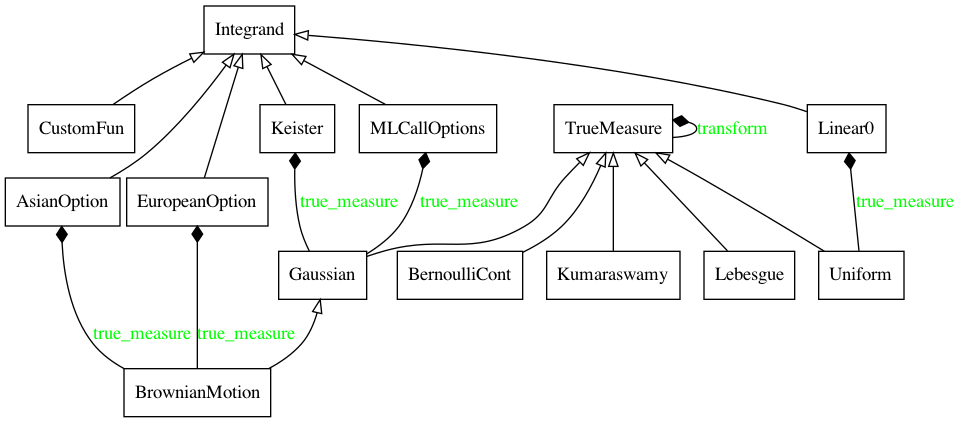
\includegraphics[width=1\textwidth]{uml/qmcpy_uml1.png}      
\end{center}   

The second UML class diagram is \texttt{DiscreteDistribution} and its subclasses.

\begin{center}
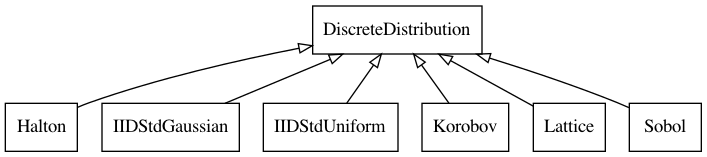
\includegraphics[width=0.7\textwidth]{uml/qmcpy_uml2.png}      
\end{center} 

The last high-level diagram relates \texttt{StoppingCriterion} and \texttt{AccumulateData}. In particular, every \texttt{StoppingCriterion} implementation uses an \texttt{AccumulateData} implementation for storing the parameters that were used and set during the numerical approximation algorithm.  \SCComment{The following class diagram includes only QMC stopping criteria, but QMCPy actually also contains a number of MC stopping criteria.}

\begin{center}
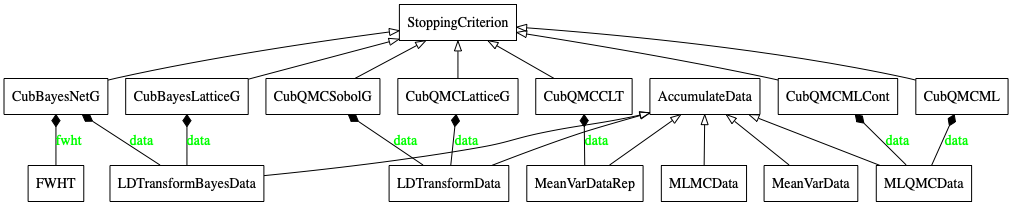
\includegraphics[width=1\textwidth]{uml/qmcpy_blog_uml3.png}      
\end{center} 


\subsection{More Details of QMCPy Classes}

In the remainder of this blog, we will present in greater detail the internal members of each main class. Each class is listed at the top of a rectangular box with its public fields and methods in the middle and bottom sections of  the box, respectively. 
%The attributes and methods are listed in alphabetical order of their names.  
A child class inherits the methods of its parent class.  However, a child's may override the parent's handed down method. In this case, the child's method is listed again at the bottom of their UML box. 

The \texttt{Integrand} class  has three main fields and methods. Each of its five subclasses has its own specific implementation of the integrand, $g$, but shares the same method, $f$, that returns the weighted average of (transformed) function at nodes from the \texttt{DiscreteDistribution}.  The specific weights, transformation, and sampling mechanism are determined by the associated realizations of the \texttt{TrueMeasure}  and \texttt{DiscreteDistribution} classes. For instance, the \texttt{Keister} integrand uses the \texttt{Gaussian} true measure and may be paired with any \texttt{DiscreteDistribution} instance.

\begin{center}
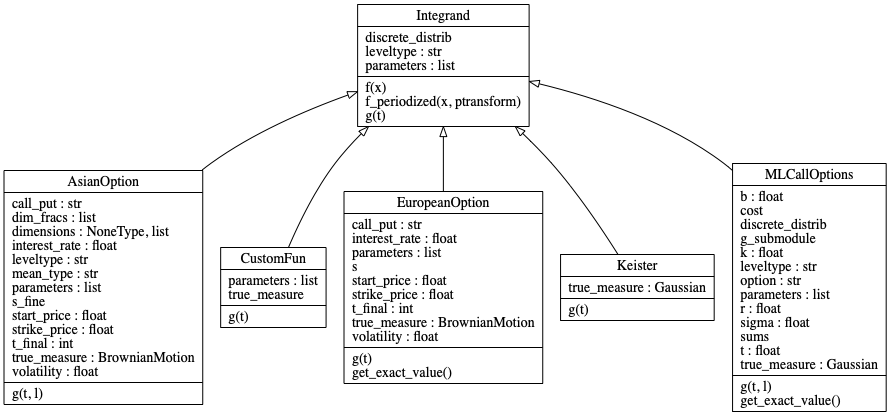
\includegraphics[width=1\textwidth]{uml/integrand_blog_uml.png}      
\end{center} 


QMCPy has implemented five children classes for \texttt{TrueMeasure}. A child class of \texttt{TrueMeasure} has an attribute called \texttt{discrete\_distrib} that is a \texttt{DiscreteDistribution} instance. This enables the main \texttt{gen\_samples()} method to select and transform points accordingly. 

\begin{center}
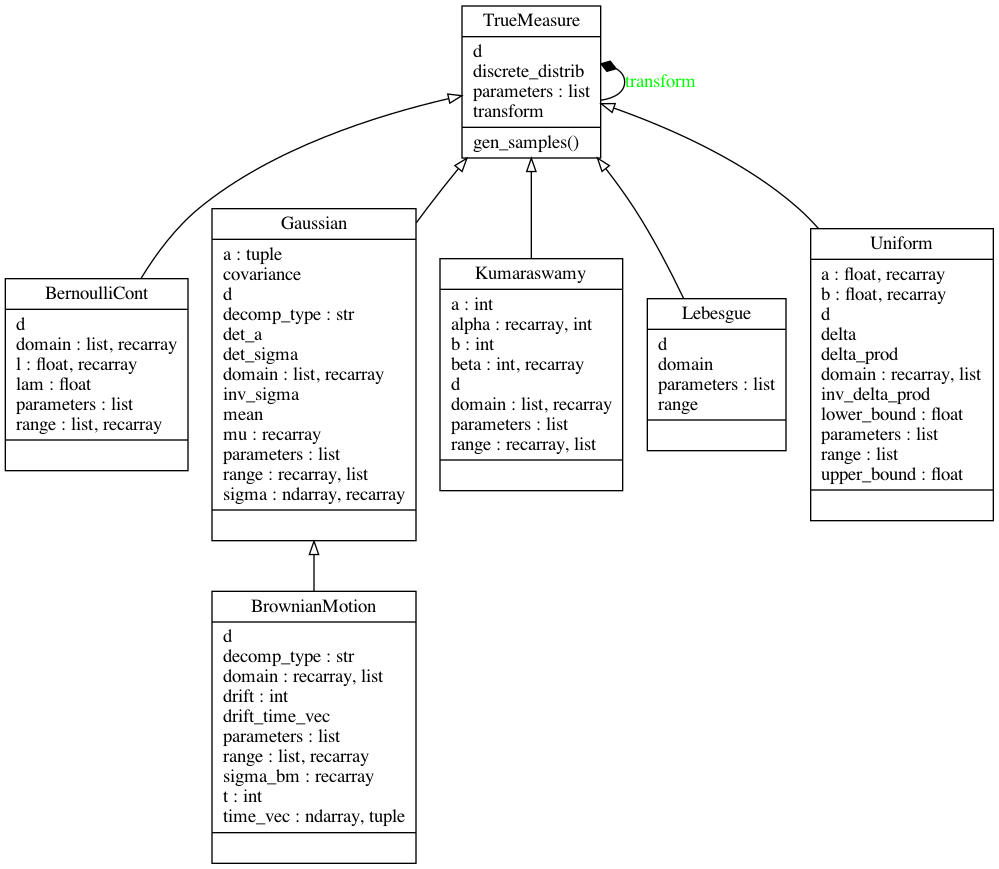
\includegraphics[width=.9\textwidth]{uml/true_measure_uml.png}  
\end{center} 

\SCComment{\texttt{DiscreteDistribution} in QMCPy plays a central role in (Q)MC algorithms, which are iterative in nature. In every iteration, a concrete subclass of \texttt{DiscreteDistribution} decides the coordinates of sampling points for integrand evaluations, which are then aggregated into an average value that serves as an estimate of a given integral problem. We refer readers to an earlier blog for a succinct presentation of  \href{https://qmcpy.org/2020/07/08/what-makes-a-sequence-low-discrepancy/}{low discrepancy sampling points} used in QMC algorithms versus IID sampling schemes in more traditional MC methods. } 

\begin{center}
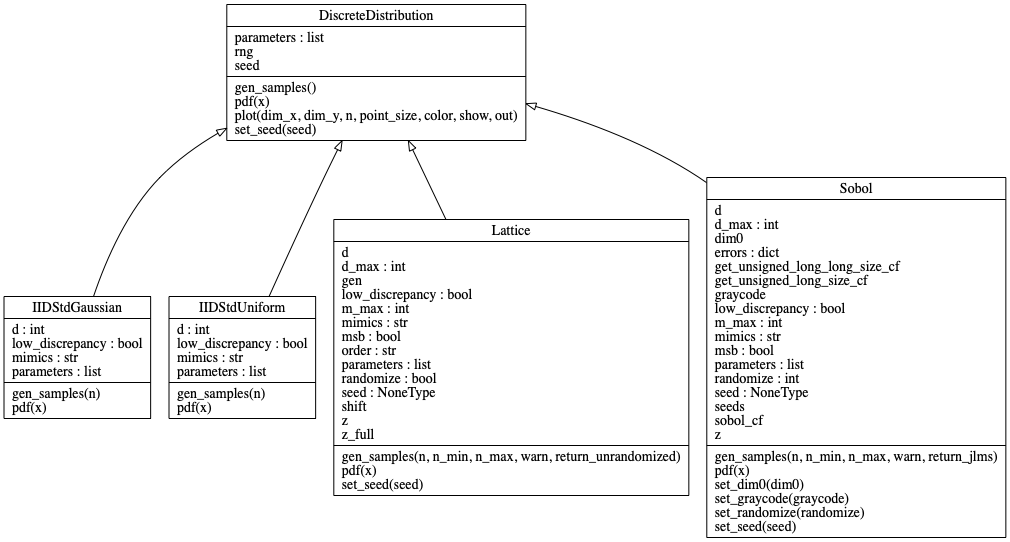
\includegraphics[width=1\textwidth]{uml/discrete_distribution_blog_uml.png} \end{center} 

QMCPy's abstract \texttt{StoppingCriterion} class currently has the largest number of instance. Each concrete implementation has two main abstract methods, \texttt{set\_tolerance()} and \texttt{integrate()}. The method \texttt{set\_tolerance()}  allows users to reset absolute and/or relative tolerances used in the \texttt{integrate()} method. Calling \texttt{integrate()} will construct an \texttt{AccumulateData} object to generate and house data such as sampling indices, function evaluations, and expectation approximations.

\begin{center}
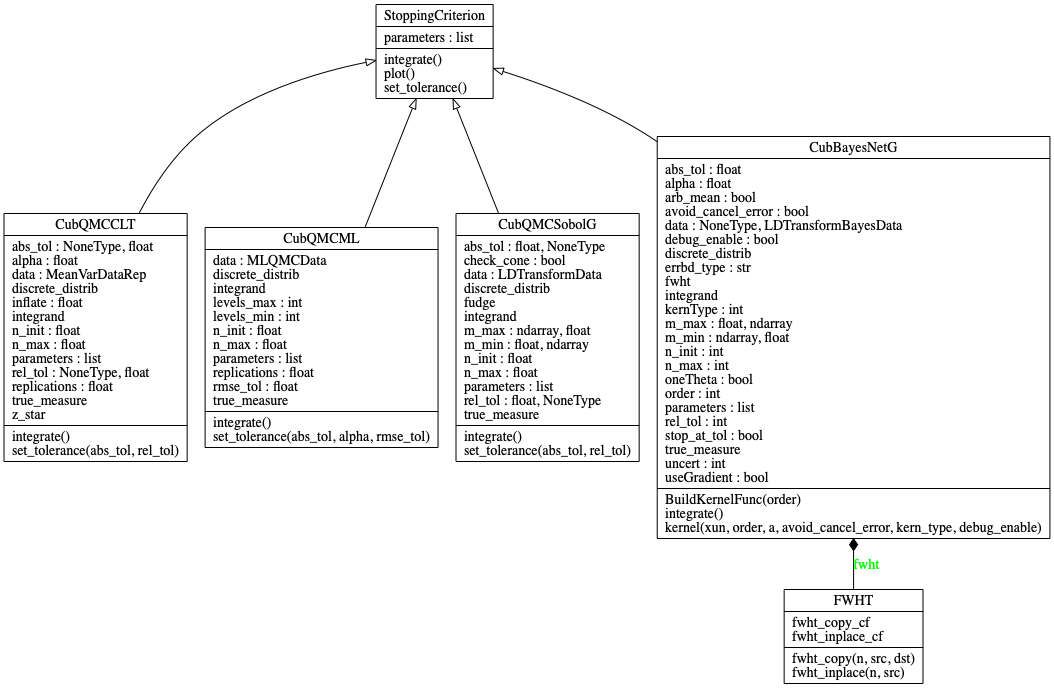
\includegraphics[width=1\textwidth]{uml/stopping_criterion_blog_uml.png}  
\end{center} 


As mentioned, an \texttt{AccumulateData} subclass collects data throughout the numerical integration computation. The method \texttt{update\_data()} collects statistical estimates such as the sample mean, sample variance, and approximate time per sample. An \texttt{AccumulateData} instance can often be used by multiple \texttt{StoppingCriterion}. For example, \texttt{LDTransformData} is used by both the \texttt{CubQMCLatticeG} and \texttt{CubQMCSobolG} stopping criteria. Since an \texttt{AccumulateData} object knows about the four other components in the QMC problem, printing the data object displays a nice summary of all relevant fields and parameters. 

\begin{center}
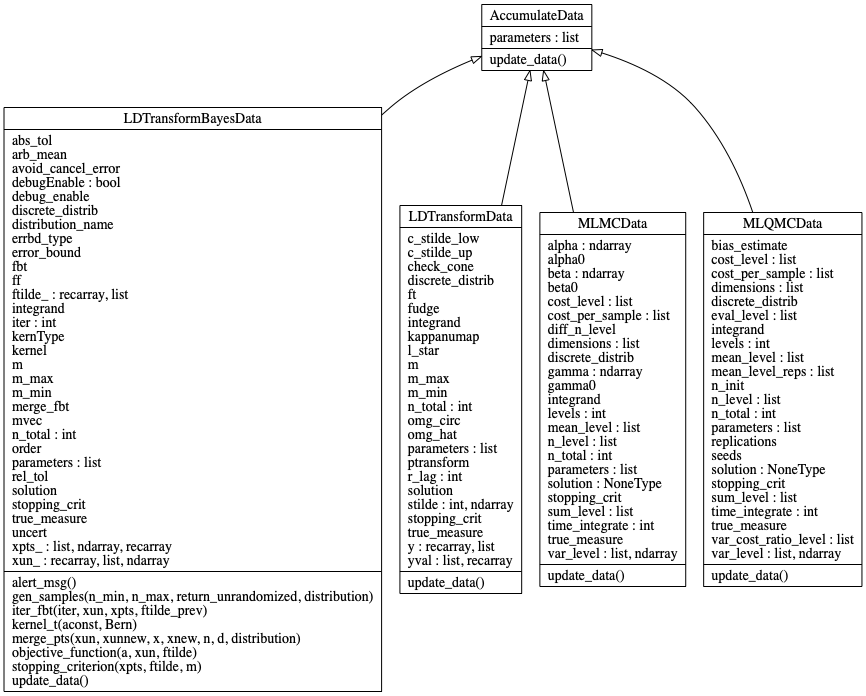
\includegraphics[width=1\textwidth]{uml/accumulate_data_blog_uml.png}  
\end{center}



Lastly, QMCPy has extended Python's \texttt{Warning} and \texttt{Exception} classes to provide developers specific types of errors and warnings. 

\begin{center}
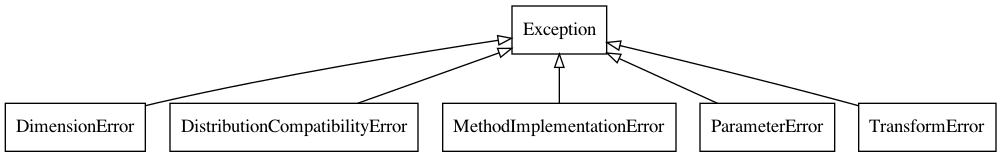
\includegraphics[width=1\textwidth]{uml/util_err.png}  
\\ 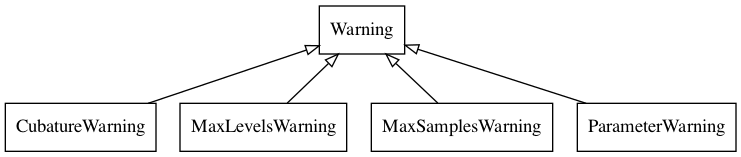
\includegraphics[width=.7\textwidth]{uml/util_warn.png}  
\end{center}

We hope these UML diagrams help both researchers and developers better understand the QMCPy architecture. The diagrams throughout this blog are reproducible using the \texttt{pyreverse} package  whose \textbf{S} option will reveal extra details including private fields and methods.
